\documentclass{article}

% https://tex.stackexchange.com/questions/106988/package-for-drawing-rdf-graphs
% https://tex.stackexchange.com/questions/9442/how-to-draw-lines-around-multiple-table-cells

% ALEPH
% http://www.cs.ox.ac.uk/activities/machlearn/Aleph/aleph_toc.html

% WARMeR
% https://arxiv.org/abs/cs/0206023

\title{
AMIE+\\
\large
Preliminary Notes\\
of the\\
Thesis Project
}

\author{Omar Trinidad Guti\'errez M\'endez}
%\institute{Informatik IV, Universitaet Bonn,}

\usepackage{amsmath}
\usepackage[utf8]{inputenc}
\usepackage{graphicx}
\usepackage[x11names]{xcolor}
\usepackage{booktabs}
\usepackage{afterpage}
\usepackage{listings}
\usepackage{floatrow}
\usepackage{float}
\usepackage{caption}

\usepackage{tikz}
    \usetikzlibrary{shapes.geometric, backgrounds, calc}
    \usetikzlibrary{arrows}
    \usetikzlibrary{arrows.meta}
    \usetikzlibrary{positioning}
    \usetikzlibrary{chains}

\usepackage{venndiagram}
\usepackage{subfig}
\usepackage[font=small]{caption}

\newcommand{\triple}[3]{{\itshape\textless#1\textgreater} {\bfseries#2} {\itshape\textless#3\textgreater}}
\newcommand{\instantiation}[2]{{\itshape#1}{$\implies$}{\itshape#2}}
\newcommand{\ins}[2]{{#1}{\implies}{#2}}
\newcommand{\body}{\vec{B}}
\newcommand{\K}{\mathcal{K}}
\newcommand{\KB}{KB $\mathcal{K}$}

%arg min
\newcommand{\argmin}[1]{\underset{#1}{\operatorname{arg}\,\operatorname{min}}\;}

% Begin tikz section %%%%%%%%%%%%%%%%%%%%%%%%%%%%%%%%%%%%%%%%%%%%%%%%%%%%%%%%%%%

% Set up a few colours
\colorlet{green}{DarkOliveGreen3!50}
\colorlet{red}{IndianRed3!50}
\colorlet{blue}{DeepSkyBlue3!50}

% ------------------------------------------------------------------------------
% A macro for marking coordinates (specific to the coordinate naming
% scheme used here). Swap the following 2 definitions to deactivate
% marks.
\providecommand{\cmark}[2][]{%
  \begin{pgfonlayer}{marx}
    \node [nmark] at (c#2#1) {#2};
  \end{pgfonlayer}{marx}
  }
\providecommand{\cmark}[2][]{\relax}

% ------------------------------------------------------------------------------
% A few box styles
% <on chain> *and* <on grid> reduce the need for manual relative
% positioning of nodes
\tikzset{
  base/.style={draw, on chain, on grid, align=center, minimum height=1cm, font={\small}},
  notes/.style={node distance=13cm, align=right},
  diam/.style={base, diamond, aspect=2, text width=5cm},
  diam_small/.style={base, diamond, aspect=2, text width=4cm},
  proc/.style={base, rectangle, text width=7cm},
  proc_small/.style={base, rectangle, text width=8em},
  term/.style={proc, rounded corners, text width=8cm},
  % coord node style is used for placing corners of connecting lines
  coord/.style={coordinate, on chain, on grid, node distance=55mm and 75mm},
  coord_inner/.style={coordinate, on chain, on grid, node distance=35mm and 55mm},
  coord_inner_inner/.style={coordinate, on chain, on grid, node distance=25mm and 35mm},
  % nmark node style is used for coordinate debugging marks
  nmark/.style={draw, cyan, circle, font={\sffamily\bfseries}},
  % ----------------------------------------------------------------------------
  % Connector line styles for different parts of the diagram
  norm/.style={->, draw, blue},
  free/.style={->, draw, green},
  cong/.style={->, draw, red},
  it/.style={font={\small\itshape}}
}

% For every picture that defines or uses external nodes, you'll have to
% apply the 'remember picture' style. To avoid some typing, we'll apply
% the style to all pictures.
\tikzstyle{every picture}+=[remember picture]

% By default all math in TikZ nodes are set in inline mode. Change this to
% displaystyle so that we don't get small fractions.
\everymath{\displaystyle}

% Introduce a new counter for counting the nodes needed for circling
\newcounter{nodecount}
% Command for making a new node and naming it according to the nodecount counter
\newcommand\tabnode[1]{\addtocounter{nodecount}{1} \tikz \node (\arabic{nodecount}) {#1};}

%\usetikzlibrary{external}
%    \tikzexternalize[prefix=tikz/]
% End tikz section %%%%%%%%%%%%%%%%%%%%%%%%%%%%%%%%%%%%%%%%%%%%%%%%%%%%%%%%%%%%%

\begin{document}
\maketitle

\section{Introduction}

Knowledge bases (KB) have the purpose of representing and store knowledge in a
machine-readable format. These databases are populated with entities and facts.

Some well-known KBs are DBpedia~\cite{dbpedia-swj}, NELL,
YAGO~\cite{suchanek2007yago}, or Freebase~\cite{bollacker2008freebase}.

A usual task executed in these databases is mining logical rules (Horn rules), that is, find
unknown relationships between entities. Some reasons why we want to obtain
logical rules are

\begin{itemize}
    \item Obtaining new facts.
    \item Identify potential new wrong facts.
    \item Use the rules for reasoning.
    \item Find especial relationships
\end{itemize}

However, these databases are designed under the idea of Open World Assumption
(OWA), that means, if the database does not contain a fact, we are not assuming
that this fact is false, as happens under the Closed World Assumption (CWA).

Finding these relations in huge datasets, and under the OWA setting is a
challenging task. This problem was addressed by Galárraga et
al.~\cite{galarraga2013amie}  who proposed Association Rule Mining under
Incomplete Evidence (AMIE) and later suggested an improved version of the same
method that they simple named AMIE+~\cite{galarraga2015fast}.

The purpose of the current project is to explore AMIE+ and implement it in a
distributed context.

\subsection{Theoretical framework}

%~\cite{rdf}
Knowledge Bases $KB$ are collections of facts; every fact is represented by a
relation between a subject and object $r(s, o)$. In this work, we are focused
on KBs modeled using the W3C standard Resource Description Framework
(RDF). In RDF, the facts are represented as triples.

An \textit{atom} is a fact with variables at the subject and/or object. A Horn
rule is composed of a head and a body.

\begin{itemize}
    \item The head is a single atom \tikz\node [fill=green!20,draw,circle] (n3) {};
    \item The body is a set of atoms \tikz\node [fill=blue!20,draw,circle] (n1) {};
\end{itemize}

% Below we mix an ordinary equation with TikZ nodes
\begin{equation}
        \tikz[baseline]{
            \node[fill=blue!20,anchor=base] (b1)
            { $B_1$ };
        } \land
        \tikz[baseline]{
            \node[fill=blue!20,anchor=base] (b2)
            { $B_2$ };
        } \land \ldots \land
        \tikz[baseline]{
            \node[fill=blue!20,anchor=base] (b3)
            { $B_n$ };
        }
        \implies
        \tikz[baseline]{
            \node[fill=green!20,anchor=base] (head)
            { $r(x, y)$ };
        }
\end{equation}

% Draw some edges between the global nodes
\begin{tikzpicture}[overlay]
        \path[->] (n1) edge [out=-100, in=-250] (b1);
        \path[->] (n1) edge [out=-100, in=-250] (b2);
        \path[->] (n1) edge [out=-100, in=-250] (b3);
        \path[->] (n3) edge [out=0, in=-250] (head);
\end{tikzpicture}

% ¿Es relevante?
% The facts in KBs are divided in A-Box and T-Box.

\subsubsection{Incompleteness}

As was stated before, the semantic KBs operate under the CWA, that is, we
assume the facts in the database are known true facts, everything else, outside
the database is asumed to be unknown.

Going beyond, we say that the unknown facts are either true or false facts, we
want to predict the new ones.

\begin{figure}
\centering
\resizebox{7.555cm}{!}{%
    
% for drawing
\def\firstellip{(0, 0) ellipse [x radius=3cm, y radius=3cm, rotate=50]}
\def\bounding{(-5,-3) rectangle (5,4)}

\begin{tikzpicture}

    \filldraw[fill=black, opacity=0.2] \bounding;

    %\scope \fill[white] \fourthellip; \endscope \filldraw[fill=red, opacity=0.2] \fourthellip;

    %single colors
    \scope
        \fill[white] \firstellip;
    \endscope

    \draw \firstellip node [label={[xshift=1.333cm, yshift=0.999cm]All here is true}] {};
    \draw \firstellip node [label={[xshift=1.333cm, yshift=2.999cm]All here is unknown}] {};

   % \draw \secondellip node [label={[xshift=2.2cm, yshift=2.1cm]$B$}] {};
   % \draw \thirdellip node [label={[xshift=-2.0cm, yshift=-0.9cm]$C$}] {};
   % \draw \fourthellip node [label={[xshift=-2.2cm, yshift=2.1cm]$D$}] {};
     \draw \bounding node [label=above left:$U$] {};

   % \begin{scope}
   %     \begin{scope}[even odd rule]% first ellipse corner
   %         \clip \secondellip (-5,-5) rectangle (5,5);
   %         \clip \thirdellip (-5,-5) rectangle (5,5);
   %         \clip \fourthellip (-5,-5) rectangle (5,5);
   %     \fill[yellow] \firstellip;
   %     \end{scope}
   % \end{scope}

   % \begin{scope}
   %     \begin{scope}[even odd rule]% second ellipse corner
   %         \clip \firstellip (-5,-5) rectangle (5,5);
   %         \clip \thirdellip (-5,-5) rectangle (5,5);
   %         \clip \fourthellip (-5,-5) rectangle (5,5);
   %     \fill[yellow] \secondellip;
   %     \end{scope}
   % \end{scope}

   % \begin{scope}
   %     \begin{scope}[even odd rule]% third ellipse corner
   %         \clip \secondellip (-5,-5) rectangle (5,5);
   %         \clip \firstellip (-5,-5) rectangle (5,5);
   %         \clip \fourthellip (-5,-5) rectangle (5,5);
   %     \fill[yellow] \thirdellip;
   %     \end{scope}
   % \end{scope}

\end{tikzpicture}

}
\caption{Incompleteness}
\label{fig:kb}
\end{figure}

\subsubsection{Rule Mining}

\subsubsection{Significance: Support and Head Coverage}

We look for meaningful rules, we have two measures of \textit{rule significance}:
support and head coverage. The \textbf{support} is the number of instantiations or
correct predictions of some rule, it is defined as

\begin{equation}
    \label{eq:support}
    supp(\vec{B} \implies r(x, y)) = \#(x, y): \exists z_1,\ldots,z_m : \vec{B} \land r(x, y) \,,
\end{equation}

\noindent where $z_1, \ldots, z_m$ are the variables of the rule that are not
$x$ and $y$. Let's consider as example the rule

\begin{equation*}
    R = \ins{livesIn(x, y)}{wasBornIn(x,y)}
\end{equation*}

\noindent and the tiny knowledge base presented in~\ref{table:significance}; we can see that
the rule is instantiated only once, \instantiation{livesIn(Bart, Springfield)}{wasBornIn(Bart, Springfield)}.

\begin{table}[ht]
    \centering
    \begin{tabular}{ c c }
    \toprule
        livesIn & wasBornIn \\
    \midrule
        \tabnode{(Bart, Springfield) } & \tabnode{(Bart, Springfield)} \\
        (Willy, Springfield)           & (Apu, India)                  \\
        (Homer, Springfield)           & \tabnode{(Willy, Scotland)}   \\
    \bottomrule
    \end{tabular}
    \caption{Tiny knowlege base}
    \label{table:significance}
\end{table}

A better way to measure the significance, is using the \textbf{head coverage}, defined as

\begin{equation}
    \label{eq:hc}
    hc(\vec{B} \implies r(x, y)) = \dfrac{supp(\vec{B} \implies r(x, y))}{size(r)} \,,
\end{equation}

\noindent where $size(r)$ is the number of times that the head rule it does
appear in the knowledge base, in the example above, \textit{wasBornIn} is
repeated two times, hence, $hc(R) = 1/3$.

\subsubsection{Confidence: Standard confidence and PCA confidence}

\begin{table}[]
    \centering
    \begin{tabular}{ c c }
    \toprule
        livesIn & wasBornIn \\
    \midrule
        \tabnode{(Bart, Springfield)}  & \tabnode{(Bart, Springfield)} \\
        \tabnode{(Willy, Springfield)} & (Apu, India)                  \\
                 (Homer, Springfield)  & (Willy, Scotland)             \\
        \tabnode{(Bart, Shellbyville)} &                               \\
    \bottomrule
    \end{tabular}

    \caption{
        Framed in red, is the entire set of conclusions that comply
        with the specified body $\body$; framed in blue, is the fact
        considered to be true; in green, all the remaining facts, negative in the CWA and
        unknown in the OWA. In brown, the facts negative facts in the PCA.
    }

    \label{table:confidence}
\end{table}

\begin{tikzpicture}[overlay]
    % some options common to all the nodes and paths
    \tikzstyle{every picture}+=[remember picture,baseline]
    \tikzstyle{every node}+=[inner sep=0pt,anchor=base,
    minimum width=1.8cm,align=center,text depth=.25ex,outer sep=1.5pt]
    \tikzstyle{every path}+=[thick, rounded corners]

    % Define the circle paths
    \draw [blue] (1.north west) -- (2.north east) --
                 (2.south east) -- (1.south west) --
                 cycle;
    \draw [red] (2.north west) -- (2.north east) --
                (3.south east) -- (3.south west) --
                cycle;
    \draw [blue] (4.north west) -- (5.north east) --
                 (5.south east) -- (4.south west) --
                 cycle;
    \draw [red] (4.north west) -- (4.north east) --
                (7.south east) -- (7.south west) --
                cycle;
    \draw [green] (6.north west) -- (6.north east) --
                  (7.south east) -- (7.south west) --
                  cycle;
    %labels
    \node [right=2.333cm, minimum width=1pt] at (2) (A) {$supp$};
    \draw [<-, out=5, in=180] (2) to (A);
    \node [right=2.333cm, minimum width=1pt] at (3) (A) {$size(r)$};
    \draw [<-, out=5, in=180] (3) to (A);
    \node [right=2.333cm, minimum width=1pt] at (5) (C) {$size(r)$};
    \draw [<-, out=5, in=180] (5) to (C);
\end{tikzpicture}

The confidence measures are used to determine the quality of a rule. The
\textbf{standard confidence} defined as

\begin{equation}
    \label{eq:stand_conf}
    conf(\vec{B} \implies r(x, y)) =
             \dfrac{supp(\vec{B} \implies r(x, y))}
                   {\#(x, y): \exists z_1,\ldots,z_m : \vec{B}} %\,,
\end{equation}

\noindent is usually used in association rule mining in the context of market basket
analysis and suppose a CWA universe, this setting is different to the one we are dealing with, but is a good reference. In AMIE, was proposed the \textbf{PCA
confidence}, to deal with the rule mining problem in an OWA universe.

\begin{equation}
    \label{eq:pca_conf}
    conf_{pca}(\vec{B} \implies r(x, y)) =
                    \dfrac{supp(\vec{B} \implies r(x, y))}
                          {\#(x, y): \exists z_1,\ldots,z_m, y' :\vec{B} \land r(x, y')} \,,
\end{equation}

%
% Improve this part!!!
%
In the PCA confidence, we assume that knowing one $y$ for a given $x$ and $r$,
we know all $y$ for that $x$ and $r$.

In the shown example, we look at the body of $R$; the relation
\textit{livesIn}, it does appear four times, and the rule is instantiated
once, the corresponding fact in the instantiated rule is considered as true. If we were considering the OWA, the three remaining facts
would be marked as unknown, the same facts would be marked as false in the CWA.

In the PCA assumption, the main purpose is to identify counter-examples from
the set of unknown facts, in the example, we see that the fact
\textit{livesIn(Bart, Shelbyville)} is contradicting the fact
\textit{livesIn(Bart, Springfield)}, which is known to be true, hence, we
consider this fact as false.

\subsubsection{Function, functionality, and inverse functionality}

The relations with \textit{at most one object} for every subject are called
\textit{functions}, for example,

\begin{itemize}
    \item \triple{Bart}{hasBirtdate}{1980} or
    \item \triple{Lisa}{hasBiologicalMother}{Marge}.
\end{itemize}

There are other type of relations, which properly, are not functions, but are
alike functions, for example,

\begin{itemize}
    \item \triple{Bart}{hasNationality}{USA} or
    \item \triple{Jurassic Park}{wasDirectedBy}{Steven Spielberg}.
\end{itemize}

Most of the movies have only one director and most of the people have one
nationality, so, the behavior of these relations is \textit{almost like a
function}. But, there are exceptions to the rule, e. g.,

\begin{itemize}
    \item \triple{Jim Carrey}{hasNationality}{Canada} and
    \item \triple{Jim Carrey}{hasNationality}{USA}. Or
    \item \triple{Poltergeist}{wasDirectedBy}{Tobe Hooper} and
    \item \triple{Poltergeist}{wasDirectedBy}{Steven Spielberg}.
\end{itemize}

So, these relations are not functions. Nevertheless, we say that have a high
degree of \textit{functionality}, which is expressed with the next equation:

\begin{equation} %\label{eq:functionality}
    fun(r) = \dfrac{\#x : \exists y : r(x, y)}{\#(x, y) : r(x, y)} \,.
\end{equation}

\noindent Another related concept is \textit{inverse functionality} $ifun(r) =
fun(r^{-1})$, in the inverse functions, every object have at most one subject,
e. g.,

\begin{itemize}
    \item \triple{Marge}{hasDaughter}{Lisa}, here, \textbf{hasDaughter}$^{-1}$ = \textbf{hasMother}.
\end{itemize}

In AMIE, it is assumed that functionality is usually higher than the inverse
functionality.

%\begin{equation} \label{eq:functionality}
%    fun(r)
%\end{equation}

\subsubsection{Language bias}

In order to limit the size of the search space, AMIE uses constraints that are called
\textit{language bias}.

% ToDo
% Tikz figure showing examples of rules.

There is an aim to limit the size of the search space, with AMIE, for example,
we use constraints on the structure of the mined rules, this is called language
bias. The idea is to have good designed language bias to avoid to deal with an
intractable search space but at the same time to generate more expressive rules.

\begin{itemize}
    \item We aim for connectivity, two atoms in a rule are connected if they share a variable or
entity. A rule is connected when every atom is connected transitively to the
rest of atoms.
    \item The rules have to be closed.
    \item Also, reflexive rules are discarded.
\end{itemize}

\subsection{Similar works}

The task of finding new logical rules given a KB has been addressed from
multiple angles. For example, ILP based approaches, relational machine learning
or hybrid approaches.

One advantage, from AMIE over relational machine learning approaches, is that
AMIE has better interpretability, which is a crucial in the Data Science world.
So, with AMIE, it is possible to mine logical rules where there is a
correlation in the data.

\section{AMIE algorithm}

% The purpose of AMIE is to generate Horn rules.
%\subsubsection{Completeness}
%Lets say that $KB*$ contains every fact of the world.

AMIE+ receives four parameters, the knowledge base KB $\mathcal{K}$, the
minimum head coverage $minHC$, the maximum size of the rules $maxLen$, and the
threshold in the confidence $minConf$. 

A queue $q$ is initialized with all the head atoms $r(x,y)$, in the same way, a
list $out$ is initialized to save the result. See the flowchart of the
algorithm in figure~\ref{fig:amie}. 

Iteratively, the rules in $q$ are dequeued; the algorithms evaluates each rule
to verify that are accepted for output (see~\ref{ssec:filter_output}), if so, it
is added to the list $out$.

When the lenght of the rule is below the $maxLen$ threshold, the refinement
is executed. In the refinement process, 

% consider this!
% https://blogs.gnome.org/muelli/2011/04/perfectly-scale-an-image-to-the-rest-of-a-page-with-latex/
\afterpage{%
\begin{figure}[p]
\centering
    \floatbox[{\capbeside\thisfloatsetup{capbesideposition={right,top},capbesidewidth=4cm}}]
    {figure}[\FBwidth]
    {\resizebox{!}{0.90\textheight}{%
            % -------------------------------------------------
% Set up a new layer for the debugging marks, and make sure it is on
% top
% this is a good example: https://tex.stackexchange.com/questions/254136/how-do-i-fix-spacing-on-paths-for-a-nested-tikz-flowchart

\pgfdeclarelayer{marx}
\pgfsetlayers{main,marx}
% A macro for marking coordinates (specific to the coordinate naming
% scheme used here). Swap the following 2 definitions to deactivate
% marks.
\providecommand{\cmark}[2][]{%
  \begin{pgfonlayer}{marx}
    \node [nmark] at (c#2#1) {#2};
  \end{pgfonlayer}{marx}
  } 
\providecommand{\cmark}[2][]{\relax} 
% -------------------------------------------------

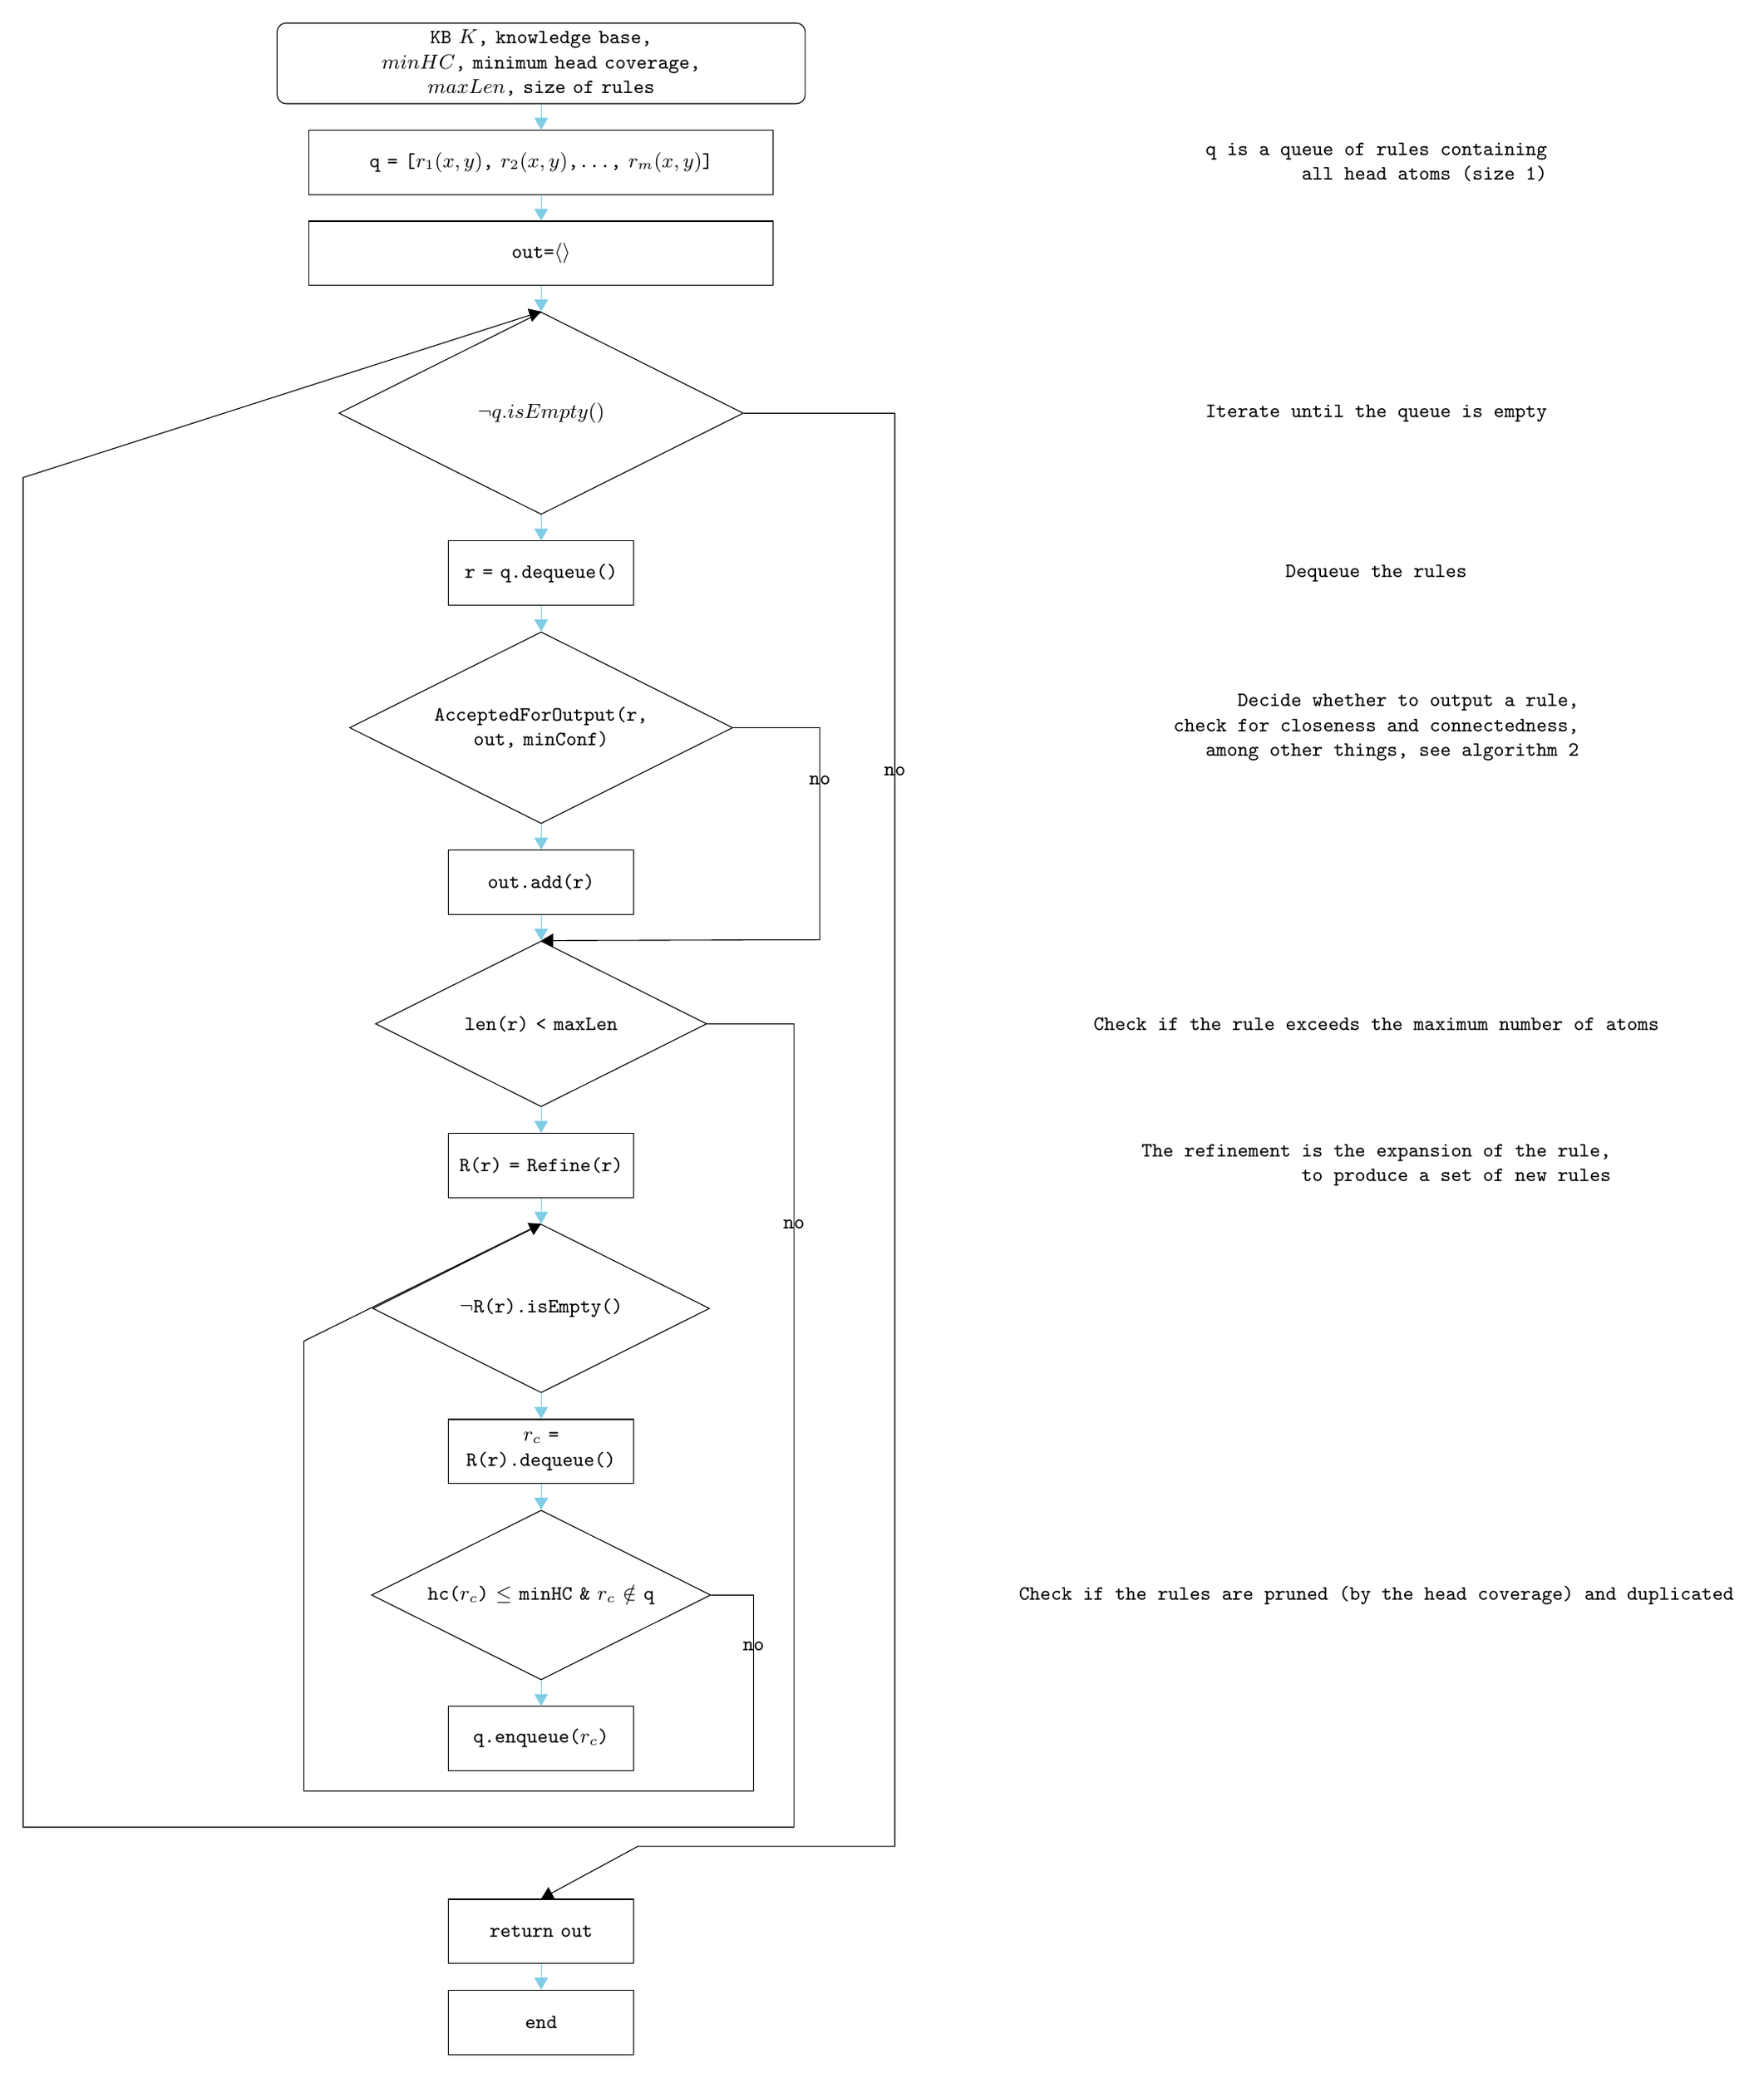
\begin{tikzpicture}[%
    >=triangle 60,              % Nice arrows; your taste may be different
    start chain=going below,    % General flow is top-to-bottom
    node distance=4mm and 10mm, % Global setup of box spacing
    every join/.style={norm},   % Default linetype for connecting boxes
    ]

{\small\ttfamily\selectfont
% ------------------------------------------------- 
% A few box styles 
% <on chain> *and* <on grid> reduce the need for manual relative
% positioning of nodes
\tikzset{
  base/.style={draw, on chain, on grid, align=center, minimum height=1cm, font={\small}},
  notes/.style={node distance=13cm, align=right},
  diam/.style={base, diamond, aspect=2, text width=5cm},
  diam_small/.style={base, diamond, aspect=2, text width=4cm},
  proc/.style={base, rectangle, text width=7cm},
  proc_small/.style={base, rectangle, text width=8em},
  term/.style={proc, rounded corners, text width=8cm},
  % coord node style is used for placing corners of connecting lines
  coord/.style={coordinate, on chain, on grid, node distance=6mm and 15mm},
  % nmark node style is used for coordinate debugging marks
  nmark/.style={draw, cyan, circle, font={\sffamily\bfseries}},
  % -------------------------------------------------
  % Connector line styles for different parts of the diagram
  norm/.style={->, draw, blue},
  free/.style={->, draw, green},
  cong/.style={->, draw, red},
  it/.style={font={\small\itshape}}
}
% -------------------------------------------------
% Start by placing the nodes
% Use join to connect a node to the previous one a

\node [term] (p0) {
    KB $K$, knowledge base,\\
    $minHC$, minimum head coverage,\\
    $maxLen$, size of rules
};
\node [proc, join] (q) {
    q = [$r_1(x, y)$, $r_2(x, y)$,\ldots, $r_m(x,y)$]
};
\node [proc, join] (p2) {
    out=$\langle\rangle$
};
\node [diam, join] (is_empty) {
    $\lnot q.isEmpty()$
};
\node [proc_small, join] (dequeue) {
    r = q.dequeue()
};
\node [diam_small, font={\small}, join] (accepted_for_output) {
    AcceptedForOutput(r, out, minConf)
};
\node [proc_small, join] (p6) {
    out.add(r)
};
\node [diam_small, join] (check_max_len) {
    len(r) < maxLen
};
\node [proc_small, join] (refinement) {
    R(r) = Refine(r)
};
\node [diam_small, join] (p9) {
    $\lnot$R(r).isEmpty()
};
\node [proc_small, join] (dequeue_refinement) {
    $r_c$ = R(r).dequeue()\\
};
\node [diam_small, join] (check) {
    hc($r_c$) $\leq$ minHC \& $r_c$ $\notin$ q
};
\node [proc_small, join] (p11) {
    q.enqueue($r_c$)
};
\node [proc_small, below of = p11, node distance = 2.6cm] (return) {return out};
\node [proc_small, join] (end) {end};


\draw[->] (check.east) -- ++(0.66,0) -- ++(0,-0.05) -- node [near start] {no} ++(0,-3.0) -- ++(-7,0) -- ++(0, 7) -- (p9.north);
\draw[->] (is_empty.east)  -- ++(0,0.0) -- ++(2.35,0) -- node [near start] {no} ++(0,-22.3) -- ++(-4,0) -- (return.north);
\draw[->] (accepted_for_output.east)  -- ++(0,0.0) -- ++(1.35,0) -- node [near start] {no} ++(0,-3.3) -- (check_max_len.north);
\draw[->] (check_max_len.east)  -- ++(0,0.0) -- ++(1.35,0) -- node [near start] {no} ++(0, -12.5) -- ++(-12,0) -- ++(0, 21) -- (is_empty.north);

% notes
\node [notes, right of=q] {q is a queue of rules containing\\all head atoms (size 1)};
\node [notes, right of=is_empty] {Iterate until the queue is empty};
\node [notes, right of=refinement] {The refinement is the expansion of the rule,\\to produce a set of new rules};
\node [notes, right of=dequeue] {Dequeue the rules};
\node [notes, right of=accepted_for_output] {Decide whether to output a rule,\\check for closeness and connectedness,\\among other things, see algorithm 2};
\node [notes, right of=check] {Check if the rules are pruned (by the head coverage) and duplicated};
\node [notes, right of=check_max_len] {Check if the rule exceeds the maximum number of atoms};

}
\end{tikzpicture}

        }}
    {\caption{Flowchart of \textsc{AMIE+} algorithm}\label{fig:amie}}
\end{figure}
\clearpage
}

\subsection{Refinement, rule expansion, mining operators}

% traverse = crisscross

The combination of conjunctions of atoms form a huge search space, which is
impossible to explore. In AMIE, a set of \textbf{mining operators} is used to
extend the rules iteratively and traverse the search space.

\subsubsection{Mining operators}
\subsection{Pruning strategies}

The mining operators add a new atom $r(x, y)$ to some rule $B_1 \land \ldots
\land B_n$. To do that, \textbf{count projection queries} are implemented. Not
every relation $r$ is tested, are select only those above the head-coverage threshold.

% Querying with Scala and Spark

\begin{lstlisting}[
           language=SQL,
           showspaces=false,
           basicstyle=\ttfamily,
           numbers=left,
           numberstyle=\tiny,
           commentstyle=\color{gray},
           mathescape=true
        ]
SELECT $r$, COUNT($H$)
WHERE $H \land B_1 \land \ldots \land B_n \land r(X, Y)$
SUCH THAT COUNT($H$) $\geq minHC \times size(H)$
\end{lstlisting}

\begin{itemize}
    \item $X$ and $Y$ are variables
    \item $H$ is the head
\end{itemize}

\noindent \textbf{Dangling atom operator} ($\mathcal{O}_\mathcal{D}$): We add a new atom with a
fresh variable $w$ and a shared variable with the rule, that is,

\begin{equation}
    r(X, Y) \in \{ r(x, w), r(y, w), r(w, x), r(w, y) \}\,.
\end{equation}

\noindent \textbf{Closing atom operator} ($\mathcal{O}_\mathcal{C}$): We aim to close the variables
that are open.

\noindent \textbf{Instantiated atom operator} ($\mathcal{O}_\mathcal{I}$):

\begin{equation}
    r(X, Y) \in \{ r(x, w), r(y, w), r(w, x), r(w, y) \}\,.
\end{equation}

\subsection{Filter the output}
\label{ssec:filter_output}

After dequeuing a rule $r$ from $q$ we filter those ones\ldots

\begin{itemize}
    \item that are not closed and not connected and whose confidence value is
        below that the $minConf$ threshold (blue block in Fig~\ref{fig:accepted_for_output}),
    %\item that has lower confidence than the ones stored in $out$
    \item whose refinements $B_1 \land \ldots \land B_n \land B_{n+1} \implies H$
        have equal or lower confidence than their parent
        $B_1 \land \ldots \land B_n \implies H$ (red blocks)
\end{itemize}

\begin{figure}[H]
\centering
\resizebox{!}{0.50\textheight}{%
    % -------------------------------------------------
% Set up a new layer for the debugging marks, and make sure it is on
% top
% this is a good example: https://tex.stackexchange.com/questions/254136/how-do-i-fix-spacing-on-paths-for-a-nested-tikz-flowchart

\pgfdeclarelayer{marx}
\pgfsetlayers{main,marx}
% A macro for marking coordinates (specific to the coordinate naming
% scheme used here). Swap the following 2 definitions to deactivate
% marks.
\providecommand{\cmark}[2][]{%
  \begin{pgfonlayer}{marx}
    \node [nmark] at (c#2#1) {#2};
  \end{pgfonlayer}{marx}
  } 
\providecommand{\cmark}[2][]{\relax} 
% -------------------------------------------------

\begin{tikzpicture}[%
    >=triangle 60,              % Nice arrows; your taste may be different
    start chain=going below,    % General flow is top-to-bottom
    node distance=7mm and 55mm, % Global setup of box spacing
    every join/.style={norm},   % Default linetype for connecting boxes
    ]

{\small\ttfamily\selectfont
% ------------------------------------------------------------------------------ 
% A few box styles 
% <on chain> *and* <on grid> reduce the need for manual relative
% positioning of nodes
\tikzset{
  % ----------------------------------------------------------------------------
  % Connector line styles for different parts of the diagram
  base/.style={draw, on chain, on grid, align=center, minimum height=1cm, font={\small}},
  notes/.style={node distance=13cm, align=right},
  diam/.style={base, diamond, aspect=2, text width=5cm},
  diam_small/.style={base, diamond, aspect=2, text width=4cm},
  proc/.style={base, rectangle, text width=7cm},
  proc_small/.style={base, rectangle, text width=8em},
  term/.style={proc, rounded corners, text width=8cm},
  % coord node style is used for placing corners of connecting lines
  coord/.style={coordinate, on chain, on grid, node distance=55mm and 75mm},
  % nmark node style is used for coordinate debugging marks
  nmark/.style={draw, cyan, circle, font={\sffamily\bfseries}},
  % ----------------------------------------------------------------------------
  % Connector line styles for different parts of the diagram
  norm/.style={->, draw, blue},
  free/.style={->, draw, green},
  cong/.style={->, draw, red},
  it/.style={font={\small\itshape}}
  % ----------------------------------------------------------------------------
}
% -------------------------------------------------
% Start by placing the nodes
% Use join to connect a node to the previous one a

\node [term] (p0) {
    rule $r$;\\
    $out$, ;\\
    $minC$, threshold in the confidence\\
};
\node [diam, join, fill=blue] (is_closed) {
    $\lnot isClosed(r)$ or $conf_{pca}(r) < minC$
};
\node [proc, join, fill=red] (parents) {
    $parents$ = $parentsOfRule(r, out)$
};
\node [diam, join, fill=red] (is_empty) {
    $\lnot$ parents.isEmpty()
};
\node [proc_small, join, fill=red] (parents_dequeue) {
    $r_p$ = parents.dequeue()
};
\node [diam_small, join, fill=red] (check_confidence) {
    $conf_{pca}(r) \leq conf_{pca}(r_{p})$
};

\node [proc_small] (end) {end};
\node [proc_small, left=of end] (false) { return $false$ };
\node [proc_small, right=of end] (true) { return $true$ };

% marks
\node[coord, left=of is_closed] (c0) {}; \cmark{0} 
\node[coord, right=of is_empty] (c1) {}; \cmark{1} 
\node[coord, left=of check_confidence] (c2) {}; \cmark{2} 
\node[coord, right=of check_confidence] (c3) {}; \cmark{3} 

% labels
\path (is_closed.south) to node [midway, xshift=1em] {no} (parents); 
\path (is_closed.west) to node [midway, yshift=1em] {yes} (c0); 
\draw [*->] (is_closed.west) -- (c0) -- (c2) |- (false);

\path (is_empty.south) to node [midway, xshift=2.4em] {not empty} (parents_dequeue); 
\path (is_empty.east) to node [midway, yshift=1em] {empty} (c1); 
\draw [o->] (is_empty.east) -- (c1) -- (c3) |- (true);

\path (check_confidence.west) to node [midway, yshift=1em] {yes} (c2); 
\draw [*->] (check_confidence.west) -- (c2);

\path (check_confidence.east) to node [midway, yshift=1em] {no} (c3); 
\draw [o->] (check_confidence.east) -- (c3);

\draw[->] (false.east)  -- (end.west);
\draw[->] (true.west)  -- (end.east);

}
\end{tikzpicture}

}
\caption{Diagram of the rule filtering.}
\label{fig:accepted_for_output}
\end{figure}

\subsection{In-memory database and queries}
\label{ssec:in_memory_database}

The efficient implementation of count projection queries was done implementing
an in-memory database. The database has three columns, for objects, relations,
and subjects: $O$, $R$, and $S$.

Every permutation of these columns is called \textit{fact index}. For every
fact index, we create a hash table that maps the first column to a second hash
table. The second hash table maps elements of the second column to a set of
elements in the third column.

\begin{figure}[H]
\centering
    \usetikzlibrary{shapes.multipart,positioning}
\newcommand{\fourdigits}[1]{%
\ifnum #1<10 0%
\fi%
\ifnum #1<100 0%
\fi%
\ifnum #1<1000 0%
\fi% 
\number #1
}
\tikzset{bucket/.style={draw,rectangle split,rectangle split
horizontal,rectangle split parts=#1,text width=.5cm,anchor=west},
mybox/.style={rectangle,draw,minimum width=1.5cm,minimum height=0.5cm}}
\newcommand{\mybucketfour}[7][]{
\node[bucket=4,#1] (#2){#4
\nodepart{two}
#5
\nodepart{three}
#6
\nodepart{four}
#7
};
\node[draw,above left=0pt of #2.north west,anchor=south west,fill=gray!30,
text width=.5cm,yshift=-\pgflinewidth]{\textbf{#3}};
}
\newcommand{\Connect}[3][-latex]{\draw[#1] (#2) to[out=0,in=180] (#3);
}

\begin{tikzpicture}[font=\sffamily,node distance=1.5cm]
    % directory
    \begin{scope}[xshift=-4cm,yshift=2cm]   
    \node[mybox,label=left:{S R O}, alias=directory-a] (box-a) {\textbf{S}};
    \node[mybox,below=0.2cm of box-a,label=left:{S O R}, alias=directory-b] (box-b) {\textbf{S}};
    \node[mybox,below=0.2cm of box-b,label=left:{R S O}, alias=directory-c] (box-c) {\textbf{R}};
    \node[mybox,below=0.2cm of box-c,label=left:{R O S}, alias=directory-d] (box-d) {\textbf{R}};
    \node[mybox,below=0.2cm of box-d,label=left:{O S R}, alias=directory-e] (box-e) {\textbf{O}};
    \node[mybox,below=0.2cm of box-e,label=left:{O R S}, alias=directory-f] (box-f) {\textbf{O}};
    \end{scope}
    % buckets
    \mybucketfour{RO}{R}{$o_0$}{$o_1$}{$\ldots$}{$o_n$}
    \mybucketfour[below=of RO.west,anchor=west]{OR}{O}{$r_0$}{$r_1$}{$\ldots$}{$r_n$}
    \mybucketfour[below=of OR.west,anchor=west]{SO}{O}{$r_0$}{$r_1$}{$\ldots$}{$r_n$}
    % links
    \Connect{directory-a}{RO}
    \Connect{directory-b}{OR}
    \Connect{directory-c}{SO}
    %\Connect{directory-0011}{D}
    %\Connect{directory-0100}{A2}
    %\Connect{directory-0101}{B}
\end{tikzpicture}

\caption{A diagram showing how the in-memory database is structured.}
\label{fig:db}
\end{figure}

Also, in the database we find \textit{aggregated indexes}, where the aggregated
number of facts are stored. Those indexes are subject $S$, predicate $P$, and object $O$.

\subsubsection{Queries}
\label{sssec:queries}

Already defined the database, we are interested in \textit{asking questions} to
it. There are seven types of queries:

\begin{itemize}
    \item Size,
    \item Existence,
    \item Select distinct,
    \item Count and
    \item Count projection
\end{itemize}

% http://www.cs.sjsu.edu/faculty/pearce/modules/lectures/prolog/kbase.htm
\noindent \textbf{Size}: We can determine \textit{how many times an
atom it does appear in a database}, for example, if we want to know the size of
the query \triple{x}{isParentOf}{y}, we look at the aggregated index $P$, that
stores the number of triples for every relation.

\noindent \textbf{Existence}: We want to answer if \textit{there are bindings
for a conjunctive query}. The algorithm~\ref{fig:existence_queries} leads with
this issue.

\begin{figure}[H]
\captionsetup{singlelinecheck=off}
\centering
    \floatbox[{\capbeside\thisfloatsetup{capbesideposition={right,top},capbesidewidth=5cm}}]
    {figure}[\FBwidth]
    {\resizebox{!}{0.60\textheight}{%
    % -------------------------------------------------
% Set up a new layer for the debugging marks, and make sure it is on
% top
% this is a good example: https://tex.stackexchange.com/questions/254136/how-do-i-fix-spacing-on-paths-for-a-nested-tikz-flowchart

\pgfdeclarelayer{marx}
\pgfsetlayers{main,marx}
% A macro for marking coordinates (specific to the coordinate naming
% scheme used here). Swap the following 2 definitions to deactivate
% marks.
\providecommand{\cmark}[2][]{%
  \begin{pgfonlayer}{marx}
    \node [nmark] at (c#2#1) {#2};
  \end{pgfonlayer}{marx}
  } 
\providecommand{\cmark}[2][]{\relax} 
% -------------------------------------------------

\begin{tikzpicture}[%
    >=triangle 60,              % Nice arrows; your taste may be different
    start chain=going below,    % General flow is top-to-bottom
    node distance=7mm and 55mm, % Global setup of box spacing
    every join/.style={norm},   % Default linetype for connecting boxes
    ]

{\small\ttfamily\selectfont
% ------------------------------------------------------------------------------ 
% A few box styles 
% <on chain> *and* <on grid> reduce the need for manual relative
% positioning of nodes
\tikzset{
  % ----------------------------------------------------------------------------
  % Connector line styles for different parts of the diagram
  base/.style={draw, on chain, on grid, align=center, minimum height=1cm, font={\small}},
  notes/.style={node distance=13cm, align=right},
  diam/.style={base, diamond, aspect=2, text width=5cm},
  diam_small/.style={base, diamond, aspect=2, text width=4cm},
  proc/.style={base, rectangle, text width=7cm},
  proc_small/.style={base, rectangle, text width=8em},
  term/.style={proc, rounded corners, text width=8cm},
  % coord node style is used for placing corners of connecting lines
  coord/.style={coordinate, on chain, on grid, node distance=55mm and 75mm},
  % nmark node style is used for coordinate debugging marks
  nmark/.style={draw, cyan, circle, font={\sffamily\bfseries}},
  % ----------------------------------------------------------------------------
  % Connector line styles for different parts of the diagram
  norm/.style={->, draw, blue},
  free/.style={->, draw, green},
  cong/.style={->, draw, red},
  it/.style={font={\small\itshape}}
  % ----------------------------------------------------------------------------
}
% -------------------------------------------------
% Start by placing the nodes
% Use join to connect a node to the previous one a

\node [term] (p0) {
    conjuctive query, $B_1 \land B_2 \land \ldots \land B_n$;\\
    \KB, knowledge base;\\
};

\node [term, join] (p0) {
    $q = B_1 \land B_2 \land \ldots \land B_n$
};

\node [diam, join, fill=blue] (is_one) {
    $n = 1$
};

\node [proc, join, fill=red] (parents) {
    $s = \argmin{i}{size(B_i, \K)} $
};

\node [proc, join] () {
    $q = q \setminus \{ B_s \}$
};

\node [diam, join] (is_empty) {
    instantiations\\$b_s \in B_s$
};

\node [proc_small, join, fill=red] (parents_dequeue) {
    $q' = q$ instantianted with bindings from $b_s$
};

\node [diam_small, join, fill=red] (check_confidence) {
    Exists(q', $\K$)
};

\node [proc_small, join] () {
    return $true$
};

\node [proc_small, join] (end) {end};
\node [proc_small, left=of end] (true) { return $size(B_1, \K)$ };
\node [proc_small, right=of end] (false) { return $false$ };

% marks
\node[coord, left=of is_one] (c0) {}; \cmark{0} 
\node[coord, right=of is_empty] (c1) {}; \cmark{1} 
\node[coord, left=of check_confidence] (c2) {}; \cmark{2} 
\node[coord, right=of check_confidence] (c3) {}; \cmark{3} 
\node[coord, right=of check_confidence] (c5) {}; \cmark{5} 

% labels
\path (is_one.south) to node [midway, xshift=1em] {no} (parents); 

\path (is_one.west) to node [midway, yshift=1em] {yes} (c0); 
\draw [*->] (is_one.west) -- (c0) -- (c2) |- (true);

\path (is_empty.south) to node [midway, xshift=2.4em] {not empty} (parents_dequeue); 
\path (is_empty.east) to node [midway, yshift=1em] {empty} (c1); 
\draw [o->] (is_empty.east) -- (c1) -- (c3) |- (false);

%\path (check_confidence.west) to node [midway, yshift=1em] {yes} (c2); 
%\draw [*->] (check_confidence.west) -- (c2);

%\path (check_confidence.east) to node [midway, yshift=1em] {no} (c3); 
%\draw [o->] (check_confidence.east) -- (c3);

\draw[->] (false.west) -- (end.east);
\draw[->] (true.east) -- (end.west);

}
\end{tikzpicture}

    }}
    {
        \caption[]{\textsc{Existence Queries} algorithm.
        \newline \newline The input is a conjunctive query and the knowledge base.
        \newline \newline When the query has only one atom, we use simply the function $size$ to determine if has bindings, as seen before.
        \newline \newline If not, we select the atom $B_s$ with the minumum number of instantiations, and save the remaining atoms as $q$.
        \newline \newline We traverse the instantiations $b_s$ of $B_s$.
        \newline \newline We join the instantiations to the remaining atoms $q$ and run the process recursively.
        }
    \label{fig:existence_queries}
    }
\end{figure}

\noindent \textbf{Select distinct}: In figure~\ref{fig:select_distinct} we see
another query.

\begin{figure}[H]
\centering
    \resizebox{!}{0.65\textheight}{%
    % -------------------------------------------------
% Set up a new layer for the debugging marks, and make sure it is on
% top
% this is a good example: https://tex.stackexchange.com/questions/254136/how-do-i-fix-spacing-on-paths-for-a-nested-tikz-flowchart

\pgfdeclarelayer{marx}
\pgfsetlayers{main,marx}
% A macro for marking coordinates (specific to the coordinate naming
% scheme used here). Swap the following 2 definitions to deactivate
% marks.
\providecommand{\cmark}[2][]{%
  \begin{pgfonlayer}{marx}
    \node [nmark] at (c#2#1) {#2};
  \end{pgfonlayer}{marx}
  } 
\providecommand{\cmark}[2][]{\relax} 
% -------------------------------------------------

\begin{tikzpicture}[%
    >=triangle 60,              % Nice arrows; your taste may be different
    start chain=going below,    % General flow is top-to-bottom
    node distance=7mm and 55mm, % Global setup of box spacing
    every join/.style={norm},   % Default linetype for connecting boxes
    ]

{\small\ttfamily\selectfont
% ------------------------------------------------------------------------------ 
% A few box styles 
% <on chain> *and* <on grid> reduce the need for manual relative
% positioning of nodes
\tikzset{
  % ----------------------------------------------------------------------------
  % Connector line styles for different parts of the diagram
  base/.style={draw, on chain, on grid, align=center, minimum height=1cm, font={\small}},
  notes/.style={node distance=13cm, align=right},
  diam/.style={base, diamond, aspect=2, text width=5cm},
  diam_small/.style={base, diamond, aspect=2, text width=4cm},
  proc/.style={base, rectangle, text width=7cm},
  proc_small/.style={base, rectangle, text width=8em},
  term/.style={proc, rounded corners, text width=8cm},
  % coord node style is used for placing corners of connecting lines
  coord/.style={coordinate, on chain, on grid, node distance=46mm and 55mm},
  coord_inner/.style={coordinate, on chain, on grid, node distance=35mm and 45mm},
  % nmark node style is used for coordinate debugging marks
  nmark/.style={draw, cyan, circle, font={\sffamily\bfseries}},
  % ----------------------------------------------------------------------------
  % Connector line styles for different parts of the diagram
  norm/.style={->, draw, blue},
  free/.style={->, draw, green},
  cong/.style={->, draw, red},
  it/.style={font={\small\itshape}}
  % ----------------------------------------------------------------------------
}
% -------------------------------------------------
% Start by placing the nodes
% Use join to connect a node to the previous one a

\node [term] () {
    projection variable, $x$;\\
    conjuctive query, $B_1 \land B_2 \land \ldots \land B_n$;\\
    \KB, knowledge base;\\
};
\node [term, join] () {
    $q = B_1 \land B_2 \land \ldots \land B_n$
};
\node [term, join] () {
    $s = \argmin{i}{size(B_i, \K)} $
};
\node [term, join] () {
    $result = \{\}$
};
\node [diam, join, fill=blue] (x_in_B) {
    $x \in B_s$
};

\node[coord, left=of x_in_B] (c0) {}; \cmark{0} 
\node[coord, right=of x_in_B] (c1) {}; \cmark{1} 

%%%%%%%%%%%%%%%%%%%%%%%%%%%%%%%%%%%%%%%%%%%%%%%%%%%%%%%%%%%%%%%%%%%%%%%%%%%%%%%%
% JA
%%%%%%%%%%%%%%%%%%%%%%%%%%%%%%%%%%%%%%%%%%%%%%%%%%%%%%%%%%%%%%%%%%%%%%%%%%%%%%%%

\node [diam_small, below=of c0] (yes_) {
    instantiations\\$x \in x$
};
\node [proc, join] () {
    $q' = q$ instantianted with bindings from $b_s$
};
\node [diam_small, join] (exists) {
    \textsc{exists}(q', $\K$)
};
\node [proc_small, join] (yes_result) {
    $result.add(x)$
};

%%%%%%%%%%%%%%%%%%%%%%%%%%%%%%%%%%%%%%%%%%%%%%%%%%%%%%%%%%%%%%%%%%%%%%%%%%%%%%%%
% NEIN
%%%%%%%%%%%%%%%%%%%%%%%%%%%%%%%%%%%%%%%%%%%%%%%%%%%%%%%%%%%%%%%%%%%%%%%%%%%%%%%%

\node [proc_small, below=of c1] (no_) {
    $q = q \setminus \{ B_s \}$
};
\node [diam_small, join] (b_in_B) {
    instantiations\\$b_s \in B_s$
};
\node [proc, join] () {
    $q' = q$ instantianted with bindings from $b_s$
};
\node [proc, join] (no_result) {
    $result.add(\textsc{select}(x, q', \K))$
};


% marks
\node[coord_inner, left=of yes_result] (c3) {}; \cmark{3} 
\node[coord_inner, below right=of exists] (c5) {}; \cmark{5} 

\node[coord, right=of yes_result] (c6) {}; \cmark{6} 
\node[coord_inner, left=of b_in_B] (c7) {}; \cmark{7} 

\node[coord_inner, right=of b_in_B] (c8) {}; \cmark{8} 

% ending nodes
% fail
%\node [proc, below=of yes_result] at ($(no_result)!0.5!(yes_result)$) {b};

% fail
%\path (yes_result) -- (no_result) node[midway below] (b) {b};

% fail
%\node [below right=of yes_result] (a) {};
%\node [below left=of no_result] (b) {};
%\node [proc, below=of yes_result] at ($(a)!0.5!(b)$) {x};
\node [proc, below=1.5cm of c6] (return) {return $result$};
\node [proc, join] () { end };

% labels
\path (x_in_B.west) to node [midway, yshift=1em] {yes} (c0); 
\draw [*->] (x_in_B.west) -- (c0) -- (yes_.north);

\path (x_in_B.east) to node [midway, yshift=1em] {no} (c1); 
\draw [o->] (x_in_B.east) -- (c1) -- (no_.north);

\draw [->] (yes_result.west) -- (c3) |- (yes_.west);
\draw [-o] (exists.east) -| (c5) -| (c3);

\draw [->] (no_result.west) -| (c7) -- (b_in_B.west);

\draw [->] (yes_.east) -| (return.north);
\draw [-o] (b_in_B.east) -| (c8) |- (c6);

}
\end{tikzpicture}

    }
    \caption[\textsc{Select Distinct} algorithm.]
    {\textsc{Select Distinct} algorithm.
        \newline \newline The input is a conjunctive query and the knowledge base.
        Firstly, it finds the atom $B_s$ with the minimum number of instantiations.
        \newline \newline \textbf{If the projection variable $x$ is in the atom $B_s$}. We traverse the instantiations $x$ of $x$.
        \newline \newline The atoms.
        \newline \newline \textbf{If the projection variable $x$ is NOT in the atom $B_s$}. We traverse the instantiations $x$ of $x$.
    }
    \label{fig:select_distinct}
\end{figure}

\noindent \textbf{Count}:

\noindent \textbf{Count projection}: With this type of query we determine the
relations and instances for new atoms in the refinement phase. The flowchart is
shown in Fig.~\ref{fig:select_distinct}.

As input, we have a selection variable $x$, a projection atom $R(X, Y)$ or $H$ that is
linked to a conjuctive query, we also have a threshold $k$ and the knowledge
base.

A hash table $map$ is initialized and the variable $q$ stores the atoms.

We verify that $x$ is present in the projection atom.

If it is present. We go through the instantiations of $H$, and check if the

If it is not present.

\begin{figure}[H]
\centering
    \resizebox{!}{0.65\textheight}{%
    % -------------------------------------------------
% Set up a new layer for the debugging marks, and make sure it is on
% top
% this is a good example: https://tex.stackexchange.com/questions/254136/how-do-i-fix-spacing-on-paths-for-a-nested-tikz-flowchart

\pgfdeclarelayer{marx}
\pgfsetlayers{main,marx}
% A macro for marking coordinates (specific to the coordinate naming
% scheme used here). Swap the following 2 definitions to deactivate
% marks.
\providecommand{\cmark}[2][]{%
  \begin{pgfonlayer}{marx}
    \node [nmark] at (c#2#1) {#2};
  \end{pgfonlayer}{marx}
  }
\providecommand{\cmark}[2][]{\relax}
% -------------------------------------------------

\begin{tikzpicture}[%
    >=triangle 60,              % Nice arrows; your taste may be different
    start chain=going below,    % General flow is top-to-bottom
    node distance=7mm and 55mm, % Global setup of box spacing
    every join/.style={norm},   % Default linetype for connecting boxes
    ]

{\small\ttfamily\selectfont
% ------------------------------------------------------------------------------
% Start by placing the nodes
% Use join to connect a node to the previous one a

\node [term] () {
    selection variable, $x$;\\
    a projection atom attached to a conjuctive query, $R(X, Y) \land B_1 \land B_2 \land \ldots \land B_n$;\\
    a threshold $k$;\\
    knowledge base, \KB;\\
};
\node [term, join] () {
    $map = \{\}$\\
    $q = B_1 \land B_2 \land \ldots \land B_n$
};
\node [diam, join] (x_in_B) {
    $x \in R(X, Y)$
};

\node[coord, left=of x_in_B] (c0) {}; \cmark{0}
\node[coord, right=of x_in_B] (c1) {}; \cmark{1}

%%%%%%%%%%%%%%%%%%%%%%%%%%%%%%%%%%%%%%%%%%%%%%%%%%%%%%%%%%%%%%%%%%%%%%%%%%%%%%%%
% JA
%%%%%%%%%%%%%%%%%%%%%%%%%%%%%%%%%%%%%%%%%%%%%%%%%%%%%%%%%%%%%%%%%%%%%%%%%%%%%%%%

\node [diam_small, below=of c0, fill=red] (yes_) {
    instantiations\\
    $r(x, y) \in R(X, Y)$
};
\node [proc, join, fill=red, label={a}] () {
    $q' = q$\\
    replace R by r, X by x, Y by y\\
};
\node [diam_small, join, fill=red] (exists) {
    \textsc{exists}(q', $\K$)
};
\node [proc_small, join, fill=red] (yes_result) {
    $map[x]++$
};

%%%%%%%%%%%%%%%%%%%%%%%%%%%%%%%%%%%%%%%%%%%%%%%%%%%%%%%%%%%%%%%%%%%%%%%%%%%%%%%%
% NEIN
%%%%%%%%%%%%%%%%%%%%%%%%%%%%%%%%%%%%%%%%%%%%%%%%%%%%%%%%%%%%%%%%%%%%%%%%%%%%%%%%

\node [diam_small, below=of c1, fill=green] (no_) {
    instantiations\\
    $r(x, y) \in R(X, Y)$
};
\node [proc, join, fill=green] () {
    $q' = q$\\
    replace R by r, X by x, Y by y\\
};
\node [proc, join, fill=green] () {
    $\mathcal{X} = \textsc{select}(x, q', \K)$
};
\node [diam_small, join, fill=green] (x_in_X) {
    $x \in \mathcal{X}$
};
\node [proc_small, join, fill=green] (no_result) {
    $map[x]++$
};

% marks
\node[coord_inner, left=of yes_result] (c3) {}; \cmark{3}
\node[coord_inner, below right=of exists] (c5) {}; \cmark{5}

\node[coord, below left=of x_in_X] (c6) {}; \cmark{6}

\node[coord_inner, right=of no_] (c8) {}; \cmark{8}

\node[coord_inner_inner, right=of x_in_X] (c2) {}; \cmark{2}
\node[coord_inner_inner, below=1cm of no_result] (c4) {}; \cmark{4}
\node[coord_inner, left=of no_result] (c9) {}; \cmark{9}

% ending nodes
\node [proc, below=1.5cm of c6] (return) {$map = \{ x \rightarrow n\} \in map: n \geq k$};
\node [proc, join] () {return $map$};
\node [proc, join] () {end};

% labels
\path (x_in_B.west) to node [midway, yshift=1em] {yes} (c0);
\draw [*->] (x_in_B.west) -- (c0) -- (yes_.north);

\path (x_in_B.east) to node [midway, yshift=1em] {no} (c1);
\draw [o->] (x_in_B.east) -- (c1) -- (no_.north);

\draw [dashed, -o] (yes_result.west) -- (c3);
\draw [->] (c3) |- (yes_.west);
\draw [-] (exists.east) -| (c5) -| (c3);

\draw [->] (yes_.east) -| (return.north);
\draw [-o] (no_.east) -| (c8) |- (c6);

\draw [dashed, -o] (no_result.west) -- (c9);
\draw [->] (x_in_X.east) -- (c2) |- (c4) -| (c9) |- (no_.west);

}
\end{tikzpicture}

    }
    \caption[\textsc{Count Projection} algorithm.]
    {\textsc{Count Projection} algorithm.
        \newline \newline
    }
    \label{fig:select_distinct}
\end{figure}

The algorithm returns a

\section{Improvements in AMIE+}

After the first publication, the authors introduced enhancements in the AMIE algorithm:

\begin{itemize}
    \item Speeding up the rule refinement.
    \item Speeding up the confidence evaluation.
\end{itemize}

\subsection{Speeding up rule refinement}

In order to enhance the rule refinement, some \textit{kind of stop conditions},
are applied. The first case is related to the \textbf{maximum rule length}:

\begin{itemize}
    \item If the size of the rule is \textbf{$maxLen -1$} we avoid to apply the
        dangling-atom operator $\mathcal{O}_\mathcal{D}$ because the result is a
        non-closed rule.
    \item With the same rule and having more than two non-closed variables:
        \begin{itemize}
            \item We avoid the closing atom operator $\mathcal{O}_\mathcal{C}$
                because we can only close at most two variables.
            \item We avoid the instantiation operator $\mathcal{O}_\mathcal{I}$
                because of the same reason.
        \end{itemize}
\end{itemize}

% ToDo: example
Also, we cease adding atoms when the rule becomes a \textbf{perfect rule}, that
is, when it accomplishes 100\% PCA confidence.

% ToDo: example and understand better
There is an special case, when adding a new dangling atom will not decrease the
support of a rule:

\begin{itemize}
    \item when the relation in the added dangling atom is already in the rule and
    \item there is also a variable in common.
\end{itemize}

In this escenario, adding a new atom does not restrict the support of the rule.
So, we can \textbf{simplify the projection query} ignoring the added atom.

\subsection{Speeding up confidence evaluation through confidence approximation}

\textit{Intuitevely bad} rules can lead to expensive confidence calculation. To
overcome this problem, a \textbf{confidence approximation} technique was
proposed.

There are some caveats, to take into account, when calculating an approximation:

\begin{itemize}
    \item Prunning good rules and
    \item few gaining, that is, computing approximation in cheap calculations.
\end{itemize}

Rules with a large number of bindings are the ones where we want to use the
confidence approximation.

\begin{equation}
    \label{eq:approx_stand_conf}
    \widehat{conf}_{pca}(R) = | dom(\body) \cap dom(r_h) | \cdot \# y_{per\ x}\,,
\end{equation}

In the first term, we simplify $dom(\body)$ to $dom(r_1)$, so we finish with
something like this:

\begin{equation*}
    dom(r_1) \cap dom(r_h)\,,
\end{equation*}

\noindent which for readability is rewritten as

\begin{equation*}
    ov_{dd}(r_1, r_h)\,.
\end{equation*}

\noindent We preferably see the second term

\begin{equation*}
    \#y_{per\ x}
\end{equation*}

\noindent as

\begin{equation*}
    \#{z_1}_{per\ x} \times \#{z_2}_{per\ z_1} \times \ldots \times \#y_{per\ z_n}\,.
\end{equation*}

\noindent That is, we traverse from the most to the least functional variable.
In the chain, the first term can be seen as:

\begin{equation*}
    \dfrac{ov_{rd}(directed, hasActor)}{|rng(directed)| \times fun(directed)}
\end{equation*}

\noindent and from the second variable the terms can be seen as:

\begin{equation*}
    \dfrac{1}{fun(r_2)} \cdot \dfrac{1}{ifun(r_2)} \,,
\end{equation*}

So, joining everything, the final formula can be seen as:

% not clear why
\begin{equation}
    \label{eq:approx_stand_conf_general}
    \widehat{conf}_{pca}(R) = \dfrac{ov_{dd}(r_1, r_h)}{fun(r_1)}
    \times
    \prod_{i=2}^{n} \dfrac{ov_{rd}(r_{i-1}, r_i)}{|rng(r_{i-1})|} \cdot \dfrac{ifun(r_i))}{fun(r_i)}
\end{equation}

\section{ToDo: Distributed implementation}

\subsection{Technological stack}

We use Hadoop, Spark, the SANSA stack, and Scala.

\subsection{SANSA Stack}
% Tikz figures for SANSA stack.

SANSA~\cite{lehmann-2017-sansa-iswc} is a platform whose purpose is\ldots A
similar work to SANSA is S2RDF~\cite{schatzle2016s2rdf}.

\bibliographystyle{plain}
\bibliography{notes}

\end{document}
